\documentclass[aspectratio=1610]{beamer}
\usetheme{Warsaw}
\useinnertheme{rectangles}
\useoutertheme{infolines}
\setbeamersize{text margin left=6mm,text margin right=6mm} 

\usepackage{xcolor}
\definecolor{IBMblue}{HTML}{648fff}
\definecolor{IBMviolet}{HTML}{785ef0}
\definecolor{IBMpink}{HTML}{dc267f}
\definecolor{IBMorange}{HTML}{fe6100}
\definecolor{IBMyellow}{HTML}{ffb000}
\definecolor{BleuClair}{HTML}{0078c0}
\definecolor{BleuFonce}{HTML}{222842}

\definecolor{codebg}{RGB}{240,240,240}
\definecolor{codecomment}{RGB}{0,128,0}
\definecolor{codekeyword}{RGB}{0,0,255}
\definecolor{codestring}{RGB}{255,100,0}

\setbeamercolor{palette primary}{bg=BleuFonce,fg=white}
\setbeamercolor{palette secondary}{bg=BleuFonce,fg=white}
\setbeamercolor{palette tertiary}{bg=BleuFonce,fg=white}
\setbeamercolor{palette quaternary}{bg=BleuFonce,fg=white}
\setbeamercolor{structure}{fg=BleuFonce} % itemize, enumerate, etc
\setbeamercolor{section in toc}{fg=BleuFonce} % TOC sections
% Override palette coloring with secondary
\setbeamercolor{subsection in head/foot}{bg=BleuClair,fg=white}

\usepackage[absolute,overlay]{textpos}
\usepackage{graphicx}
\usepackage[center]{caption}
\usepackage{amsfonts}
\setbeamertemplate{caption}[numbered]
\usepackage{amsmath,mathrsfs,amssymb,stmaryrd}
\usepackage{geometry}
\usepackage{pgfplots} 
\usepackage{tikz, xifthen}
\usepackage{algorithm}
\usepackage{algpseudocode}
\usepackage{animate}
\usepackage{multicol}

\usepackage{hyperref}
\usepackage[style=authoryear, backend=biber]{biblatex}
\addbibresource{biblio.bib}
\usepackage{csquotes}

\usepackage{cancel}
\usepackage{soul}
\usetikzlibrary{matrix, positioning, arrows.meta, fit}
\usepackage{fp}
\usepackage{pgfplots}
\pgfplotsset{compat=1.17}
\usepgfplotslibrary{patchplots}
\usepackage{listings}  % Ajout du package listings
\usepackage{lipsum}    % Pour le texte de remplissage (lipsum)
\usepackage[english]{babel}
\newcommand{\up}[1]{\textsuperscript{#1}}

\usepackage{empheq}

\usepackage[warnings-off={mathtools-colon,mathtools-overbracket}]{unicode-math}
%\setmainfont{Fira Sans}%
%\setsansfont{Fira Sans}
%\setmathfont{Fira Math}

\ExplSyntaxOn
\bool_gset_true:N\g__um_upGreek_bool
\bool_gset_false:N\g__um_upgreek_bool
\bool_gset_true:N\g__um_bfupGreek_bool 
\bool_gset_false:N\g__um_bfupgreek_bool 
\bool_gset_false:N \g__um_bfliteral_bool
\bool_gset_true:N  \g__um_bfupLatin_bool
\bool_gset_true:N  \g__um_upLatin_bool
\bool_gset_false:N  \g__um_bfuplatin_bool
\bool_gset_false:N  \g__um_uplatin_bool
%more if needed ...
\ExplSyntaxOff

\newcommand{\bm}[1]{\symbf{#1}}
\newcommand{\di}{\ensuremath{\, \mathrm{d}}}
\newcommand{\e}{\ensuremath{\mathrm{e}}}


% Configuration du package listings pour le langage C
\lstdefinestyle{mystyle}{
    belowcaptionskip=1\baselineskip,
    breaklines=true,
    frame=L,
    xleftmargin=3em, % Reduced left margin
    language=C,
    showstringspaces=false,
    basicstyle=\scriptsize\ttfamily, % Smaller font size
    keywordstyle=\color{codekeyword},
    commentstyle=\color{codecomment},
    stringstyle=\color{codestring},
    backgroundcolor=\color{codebg},
    numbers=left,
    numberstyle=\tiny\color{gray},
    stepnumber=1,
    numbersep=10pt, % Reduced number separation
    captionpos=b,
    tabsize=2,
    breakatwhitespace=false,
}

\lstdefinestyle{customc}{
    belowcaptionskip=1\baselineskip,
    breaklines=true,
    frame=L,
    xleftmargin=\parindent,
    language=C,
    showstringspaces=false,
    basicstyle=\footnotesize\ttfamily,
    keywordstyle=\bfseries\color{codekeyword},
    commentstyle=\itshape\color{codecomment},
    stringstyle=\color{codestring},
    backgroundcolor=\color{codebg},
    numbers=left,
    numberstyle=\tiny\color{gray},
    stepnumber=1,
    numbersep=10pt,
    captionpos=b,
    tabsize=2,
    breakatwhitespace=false,
}


\setbeamertemplate{footline}{%
	\leavevmode\hbox{%
\begin{beamercolorbox}[wd=\paperwidth, ht=4ex,dp=2ex,leftskip=.3cm]%
{author in head/foot}%
    \usebeamerfont{author in head/foot}{\normalsize\insertframenumber/\inserttotalframenumber}
    \hfill \hspace{-4cm} \hspace{2.6cm}\usebeamerfont{author in head/foot}\insertshorttitle \hfill ~
\end{beamercolorbox}%
}
  \vskip0pt}
 
 
\logo{\hspace*{-1cm}
\includegraphics[height=0.5cm]{logo-embxinp.png}}

% \colorlet{bleu_item}{blue!80!green}
% \setbeamertemplate{itemize item}[square]
% \setbeamercolor{itemize item}{fg=bleu_item}
% \setbeamertemplate{frametitle continuation}{}


\hypersetup{breaklinks=true}
\setbeamercolor{framesource}{fg=gray}
\setbeamerfont{framesource}{size=\tiny}
\newcommand{\source}[1]
{
	\begin{beamercolorbox}[ht=0cm,right]{framesource}
		\usebeamerfont{framesource}\usebeamercolor[fg]{framesource} Source: {#1}
	\end{beamercolorbox}
	\vspace{-6mm}	
}
\pdfstringdefDisableCommands{%
  \def\\{}%
  \def\texttt#1{<#1>}%
}

% Title Page
\setbeamerfont{title}{series=\bfseries,parent=structure}
\title{Resolution of the linear Boltzmann equation\\ by Monte Carlo method}
\subtitle{}

\author{Antoine Boucher\\
Gabriel Rodiere\\
Clément Aumonier\\
Guillaume Doyen\\
Khaoula El Maddah\\
Supervisor : Gael Poette} 
\institute{}
\date{Wednesday, 31\up{st} January 2024}
\titlegraphic{
\includegraphics[height=1cm]{logo-embxinp.png}}

\setbeamerfont{frametitle}{series=\bfseries,size=\large,parent=structure}

% Begin Document
\begin{document}

% Title Page
\begin{frame}[plain]
  \titlepage
\end{frame}

% Outline Slide
\begin{frame}{Table of contents}
  \tableofcontents
\end{frame}

\section{Introduction}
\begin{frame}{Fields of Application for the Boltzmann Equation}
\begin{multicols}{2}
    \begin{figure}
      \centering
      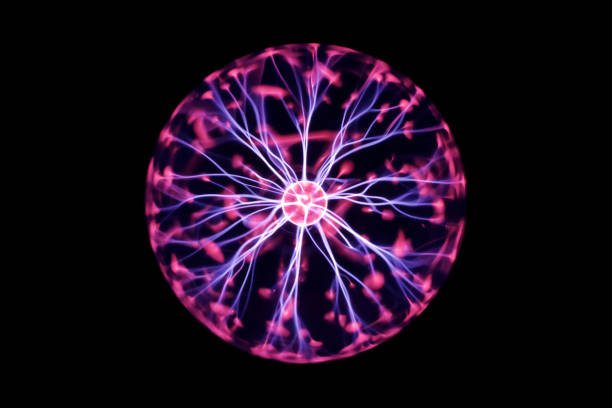
\includegraphics[width=0.6\linewidth]{plasma physics.jpg}
      \caption*{Plasma physics}
      
      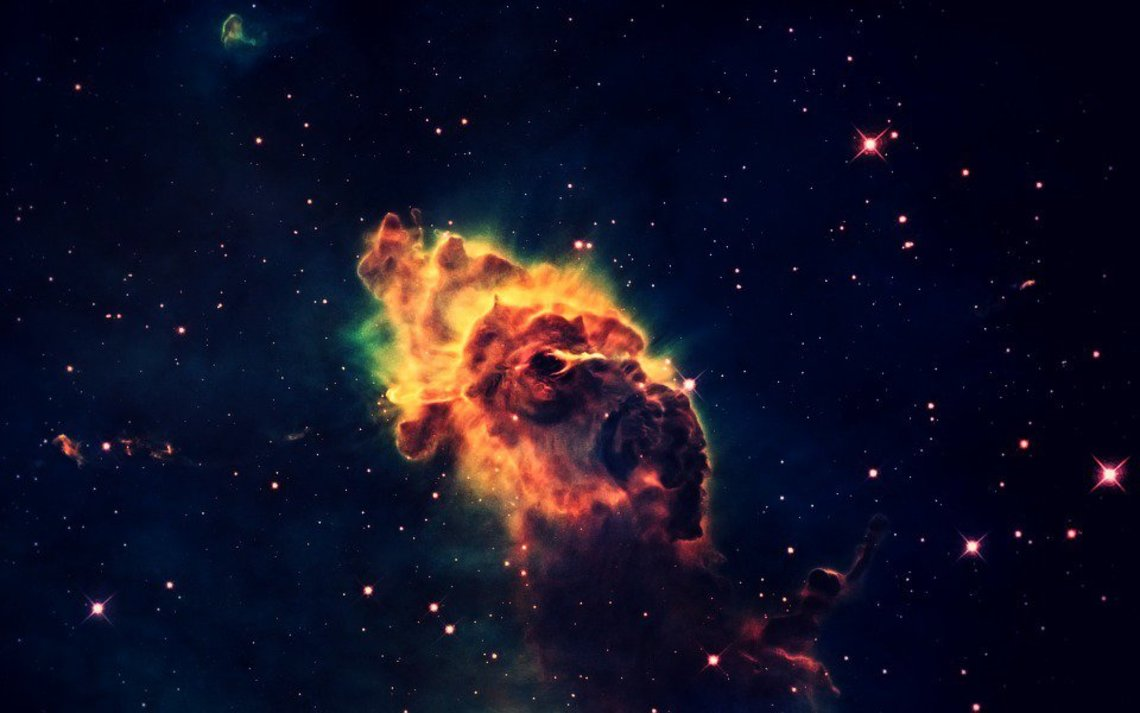
\includegraphics[width=0.6\linewidth]{astrophysics.jpg}
      \caption*{Astrophysics}
    	%\end{figure}

    %\begin{figure}
      %\centering
      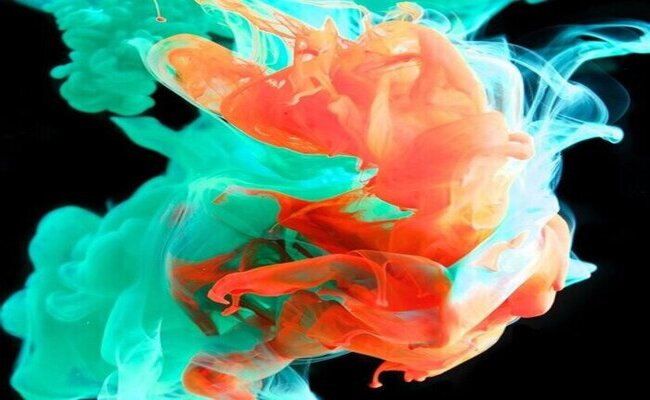
\includegraphics[width=0.6\linewidth]{dynamique_fluides-2.jpg}
      \caption*{Fluid dynamic}
      
      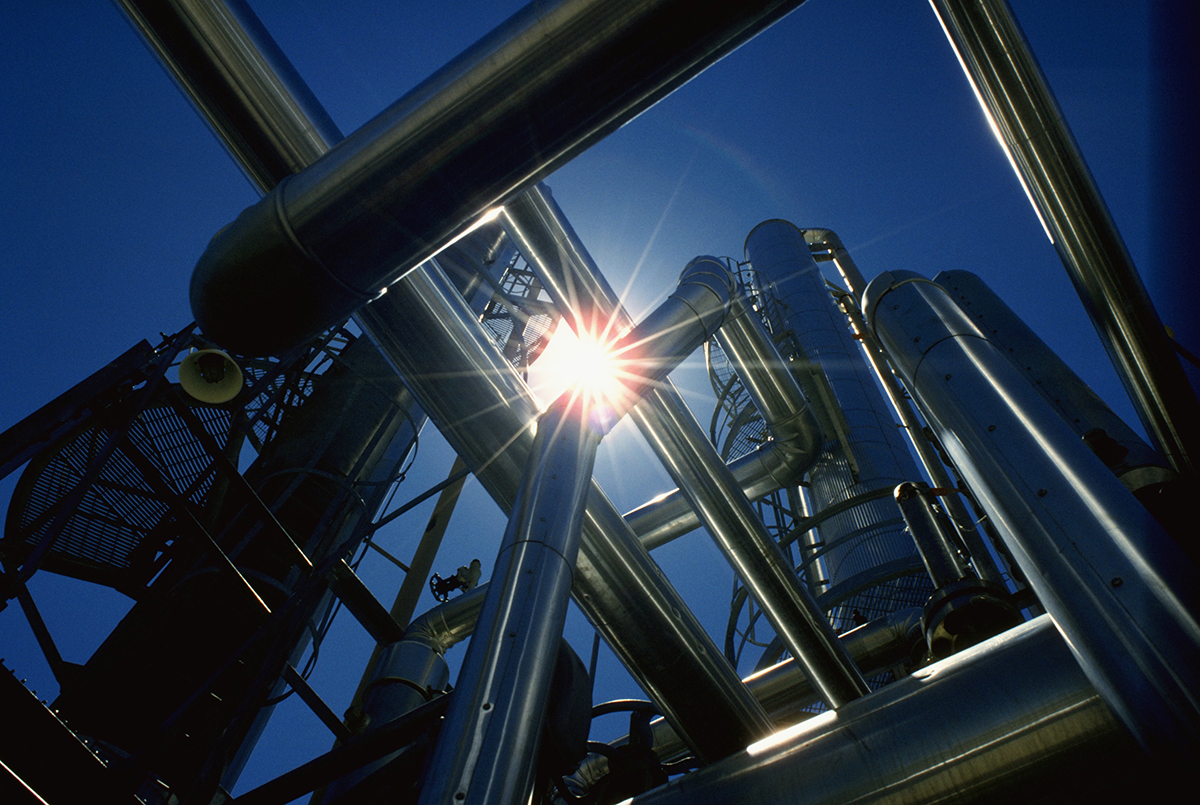
\includegraphics[width=0.6\linewidth]{gas.jpg}
      \caption*{Rarefied Gas Dynamics}
    \end{figure}
\end{multicols}
\end{frame}

\section{Monte Carlo method}
\begin{frame}{Example of the calculation of $\pi$}
We draw a circle with a radius of $r = 1$ inscribed in a square of side length 2. We throw stones in the air and count the number of stones within the circle. An estimate of $\pi$ is given by 
\begin{equation*}
    \pi_N =\frac{\text{Number of stones within the circle}}{4 N}
\end{equation*}
\begin{figure}[h]
  \centering
  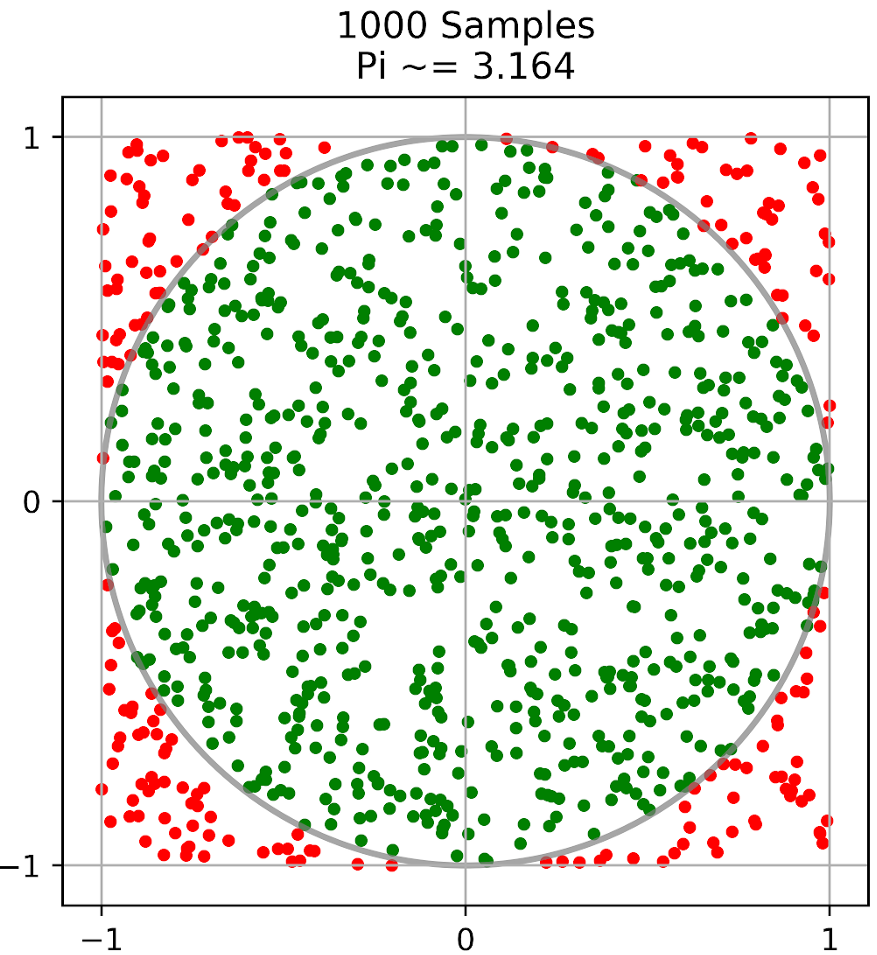
\includegraphics[height=0.5\textheight]{pi.png}
  \label{fig:circle_mc}
\end{figure}
\end{frame}


\section{The existence and uniqueness of the solution: Cauchy Problem}

\begin{frame}{Special cas with Absorption and Source Term}
We consider damping and the source term, assuming they belong to $\mathcal{C}^1(\mathbb{R}_+ \times \mathbb{R}^n)$. The considered Cauchy problem is as follows:

	
\[
\begin{cases}
\frac{\partial u}{\partial t}(t,\bm{x})+\bm{v} \cdot \nabla_{\bm{x}} u(t,\bm{x}) + a(t,\bm{x})u(t,\bm{x}) = S(t,\bm{x}), \quad \bm{x} \in \mathbb{R}^n, \quad t>0.\\
u(0,\bm{x}) = u_{0}(x)
\end{cases}
\]

In this case, if $u_0 \in \mathcal{C}^1(\mathbb{R}^n)$, then using the method of characteristics, we can still demonstrate that the Cauchy problem has a unique solution $u \in \mathcal{C}^1(\mathbb{R}_+ \times \mathbb{R}^n)$. This solution is given as follows:\\

\begin{equation*}
u(t,\bm{x}) = u_0(\bm{x}-t\bm{v}) \e^{-\int_0 ^t a(\tau, \bm{x}+(t-\tau)\bm{v}) \di \tau} + \int_0^t  \e^{-\int_0 ^t a(\tau, \bm{x}+(t-\tau)\bm{v})\di\tau} S(s,\bm{x}+(s-t)\bm{v}) \di s
\end{equation*}

    
\end{frame}



\section{Resolution of the equation}
\begin{frame}{Boltzmann equation}
    This work is based on \cite{noauthor_transport_2018}, \cite{poette:tel-02288678} \& \cite{lapeyre_methodes_1998}.
    
    The transport equation in an infinite medium with its corresponding deterministic collisional component can be expressed as:
 \begin{equation*}
\partial_t u(x,t,\bm{v}) + \bm{v} \cdot \nabla u(x,t,\bm{v}) + v\sigma_t (x,t,\bm{v})u(x,t,\bm{v})= v\sigma_s(x,t,\bm{v}) \! \int P(x,t,\bm{v},\bm{v}')u(x,t,\bm{v}') \di\bm{v}' \label{ref11}
 \end{equation*}
Where 
\begin{equation*}
   \sigma_s (x,t,\bm{v})= \int \sigma_s (x,t,\bm{v},\bm{v}') \di \bm{v}', \quad  P (x,t,\bm{v},\bm{v}')=
\frac{\sigma_s (x,t,\bm{v},\bm{v}')}{\sigma_s (x,t,\bm{v})}
\end{equation*}
$\sigma_t$ is the total cross-section

$\sigma_s$ is the scattering cross-section

$v \sigma_t$ is a damping term
\end{frame}

\begin{frame}{Variable change}
    The approach involves a series of variable changes. The initial step is re-expressing the transport equation with respect to a characteristic $x + vt$. As a result, it transforms into:
    \begin{equation*}
        \begin{split}
            \partial _s u(x+\bm{v}s,s,\bm{v}) &= -v\sigma_t (x+\bm{v}s,s,\bm{v})u(x+\bm{v}s,s,\bm{v}) \\
            &\quad + v\sigma_s(x+\bm{v}s,s,\bm{v})\int P (x+\bm{v}s,s,\bm{v},\bm{v}')u(x+\bm{v}s,s,\bm{v}')d\bm{v}'
        \end{split}
    \end{equation*}
\end{frame}

\begin{frame}{Equation Transformation with Multiplication and Integration}
    After multiplying both sides of the equation by:
    \begin{equation*}
        \e^{\int _0^s v\sigma_t (x + \bm{v}\alpha,\alpha, v) \di \alpha}
    \end{equation*}
    
    Following that, we obtain
    \begin{equation*}
    \begin{split}
        &\partial _s [u(x+\bm{v}s,s,\bm{v})\e^{\int _0^s v\sigma_t (x + \bm{v}\alpha,\alpha, v) \di \alpha}] \\
        &= \e^{\int _0^s v\sigma_t (x + \bm{v}\alpha,\alpha, v) d\alpha} v\sigma_s(x+\bm{v}s,s,\bm{v})\int P (x+\bm{v}s,s,\bm{v},\bm{v}')u(x+\bm{v}s,s,\bm{v}') \di \bm{v}'
    \end{split}
    \end{equation*}
\end{frame}

\begin{frame}{Integration of the equation}
    We get after integrating the equation between [0, t]:
    \begin{multline*}
        u(x+\bm{v}t,t,\bm{v}) = u_0(x, \bm{v}) \exp\left(- \int_{0}^{t} v\sigma_t\left(x + \bm{v} \alpha, \alpha, \bm{v}\right) \di\alpha\right) \\
        + \int_{0}^{t} \int v\sigma_s\left(x + \bm{v}s, s, \bm{v}\right) u\left(x + \bm{v}s, s, \bm{v}'\right) \e^{- \int_s^t v\sigma_t\left(x + \bm{v} \alpha, \bm{v}\right) \di\alpha} P\left(x + \bm{v} s, s, \bm{v}, \bm{v}'\right) \di\bm{v}' \di s
    \end{multline*}

     After a variable change, we obtain:
    \begin{multline*}
        u(x,t,\bm{v}) = u_0(x - \bm{v}t, \bm{v}) \exp\left(- \int_{0}^{t} v\sigma_t\left(x - \bm{v}(t - \alpha), \alpha, \bm{v}\right) \do\alpha\right) \\
        + \int_{0}^{t} \int v\sigma_s\left(x - \bm{v}(t - s), s, \bm{v}\right) u\left(x - \bm{v}(t - s), s, \bm{v}'\right) \\
        \e^{- \int_s^t v\sigma_t\left(x - \bm{v}(t - \alpha), \bm{v}\right) \di\alpha} P\left(x - \bm{v}(t - s), s, \bm{v}, \bm{v}'\right) \di\bm{v}' \di s
    \end{multline*}
\end{frame}

\begin{frame}{Re-expression of the exponential}
    We also have:
    \begin{multline*}
        \exp\left(- \int_{0}^{t} v\sigma_t\left(x - \bm{v}(t - \alpha), \alpha, \bm{v}\right) \di \alpha\right) = \exp\left(- \int_{0}^{t} v\sigma_t\left(x - \bm{v} \alpha,t- \alpha, \bm{v}\right) \di \alpha\right) \\ 
        = \int _t^\infty  v\sigma_t\left(x - \bm{v} s,t- s, \bm{v}\right)
        \exp\left(- \int_{0}^{s} v\sigma_t\left(x - \bm{v} \alpha,t- \alpha, \bm{v}\right) \di\alpha\right) \di s
    \end{multline*}
\end{frame}
\begin{frame}{The integral form of the Boltzmann equation}
    Then the integral representation of the transport equation is provided by:
    \begin{multline*}
        u(x,t,\bm{v}) =  \int _t^\infty  u_0(x - \bm{v}t, \bm{v}) v\sigma_t\left(x - \bm{v} s,t- s, \bm{v}\right) \exp\left(- \int_{0}^{s} v\sigma_t\left(x - \bm{v} \alpha,t- \alpha, \bm{v}\right) d\alpha\right) \di s\\
        + \int_{0}^{t} \int v\sigma_s\left(x - \bm{v}(t - s), s, \bm{v}\right) u\left(x - \bm{v}(t - s), s, \bm{v}'\right) \\
        \e^{- \int_s^t v\sigma_t\left(x - \bm{v}(t - \alpha), \bm{v}\right) d\alpha} P\left(x - \bm{v}(t - s), s, \bm{v}, \bm{v}'\right) \di \bm{v}' \di s \label{ref13}
    \end{multline*}

    \textbf{Problem : the solution depends on its own integral !}
    $\longrightarrow$ Let's introduce a numerical MC scheme !
\end{frame}

\section{The semi-analog MC scheme}

\begin{frame}{Semi-analog scheme}
    Developing a Monte Carlo scheme involves introducing random variables and their associated probability measure to express the equation as an expectation. The choice of this set of random variables is not unique, leading to different Monte Carlo schemes with distinct properties.

    For the semi-analog scheme, we introduce the probability measure of the interaction time: 
    \begin{equation*}
    f_{\tau}(\bm{x}, t, \bm{v}, s) \di s = 1_{[0,\infty[}(s) \, v\sigma_t(\bm{x} - \bm{v}s, t - s, v) \e^{-\int_{0}^s v\sigma_t(\bm{x} - \bm{v}\alpha, t - \alpha, v) \, \di \alpha} \di s
    \end{equation*}
    for all $(x, t, v) \in D \times [0, T] \times \mathbb{R}^3$\\
    We introduce the specified random variables corresponding to the previously identified probability measures.
    \begin{equation*}
        \left\{
            \begin{array}{ll}
                \tau \text{ with probability measure } f_{\tau}(\bm{x}, t, \bm{v}) \, \di s, \\
                \bm{V}' \text{ with probability measure } P_{\bm{V}'}^{s}(\bm{x}, t, s, \bm{v}, \bm{v}') \, \di v'
            \end{array}
        \right.
    \end{equation*}

\end{frame}
\begin{frame}{Expression of the solution}
We found the following expectation value:
    \begin{equation*}
            u(\bm{x}, t, \bm{v}) = \mathbb{E} \left[1_{[t, \infty[}(\tau) \: u_0(\bm{x} - \bm{v}t, \bm{v}) + 1_{[0, t[}(\tau) \: \frac{\sigma_s(\bm{x} - \bm{v}\tau, t - \tau, v)}{\sigma_t(\bm{x} - \bm{v}\tau, t - \tau, v)}u(\bm{x} - \bm{v}\tau, t - \tau, \bm{V}')\right]
    \end{equation*}
Essentially, the process of constructing a Monte Carlo scheme is based on searching for solutions of expectation that possess this specific structures:
\begin{equation*}
u_p(\bm{x},t,\bm{v}) = w_p(t)\: \delta_x(\bm{x}_p(t)) \:\delta_{\bm{v}}(\bm{v}_p(t)) 
\end{equation*}
Replacing \(u_p\) in the equation yields:
\begin{empheq}[left=\empheqbiglbrace]{align*}
w_p(t) &= 1_{[0,\infty[}(\tau)w_p(0) + 1_{[0,t[}(\tau) \frac{\sigma_s}{\sigma_t} \left( x_p(t-\tau),t-\tau,\bm{v}_p(t-\tau) \right) w_p(t-\tau),\\
x_p(t) &= 1_{[0,\infty[}(\tau)(\bm{x}_0-\bm{v}t) + 1_{[0,t[}(\tau)(x_{t-\tau}-\bm{v}\tau),\\
v_p(t) &= 1_{[0,\infty[}(\tau)\bm{v} + 1_{[0,t[}(\tau)\bm{V}'. 
\end{empheq}

\end{frame}
%\begin{frame}{Algorithm}
\begin{frame}[fragile]{Monte Carlo Particle Transport Algorithm}
    \begin{multicols}{2}
        \begin{algorithmic}[1]
                \State Let $u(\bm{x}, t, \bm{v}) \gets 0$;
                \For{$p \in \llbracket 1 ; N_{MC} \rrbracket$}
                    \State set $s_p = t$
                    \State set $\bm{x}_p = \bm{x}$
                    \State set $\bm{v}_p = \bm{v}$
                    \State set $w_p(t) = N_{MC}$
                    \While{$s_p > 0$ and $w_p > 0$}
                        \If{$\bm{x}_p \not \in \mathcal{D}$}
                            \State apply\_BCs$(\bm{x}_p, s_p, \bm{v}_p)$
                        \EndIf
                        \State $\tau \gets P \leadsto f_\tau(\bm{x}_p, s_p, s, \bm{v}_p) \di s$
                        \newcolumn
                        \If{$\tau > s_p$}
                            \State $\bm{x}_p \gets \bm{x}_p + s_p \bm{v}_p$
                            \State $s_p \gets 0$
                            \State $u(\bm{x}, t, \bm{v}) += w_p u_0(\bm{x}_p, \bm{v}_p)$
                        \Else
                            \State $w_p \gets \frac{\sigma_s(\bm{x}_p, s_p - \tau, \bm{v}_p)}{\sigma_t(\bm{x}_p, s_p - \tau, \bm{v}_p)} w_p$
                            \State $\bm{v}_p \gets \bm{V}' \leadsto P_{\bm{V}'}s(\bm{x}_p, s_p, \tau, \bm{v}_p, \bm{v}') \di \bm{v}'$
                            \State $\bm{x}_p \gets \bm{x}_p + \bm{v}_p \tau$
                            \State $s_p \gets s_p - \tau > 0$
                        \EndIf
                    \EndWhile

                \EndFor
        \end{algorithmic}
    \end{multicols}
\end{frame}

\section{Numerical results}

\begin{frame}[fragile]{Sampling of $\tau$ and $\bm{v}_p$}
    $\tau = - \frac{\log U}{\sigma_t(\bm{x}_p, s_p, \bm{v}_p) |\bm{v}_p|}$ where $U \leadsto U[0;1]$.

    $\bm{v}_p$ is sampled uniformly on the 3D unit sphere.
    \vspace{-1em}
    \begin{figure}[h]
  \centering
  \begin{multicols}{2}
  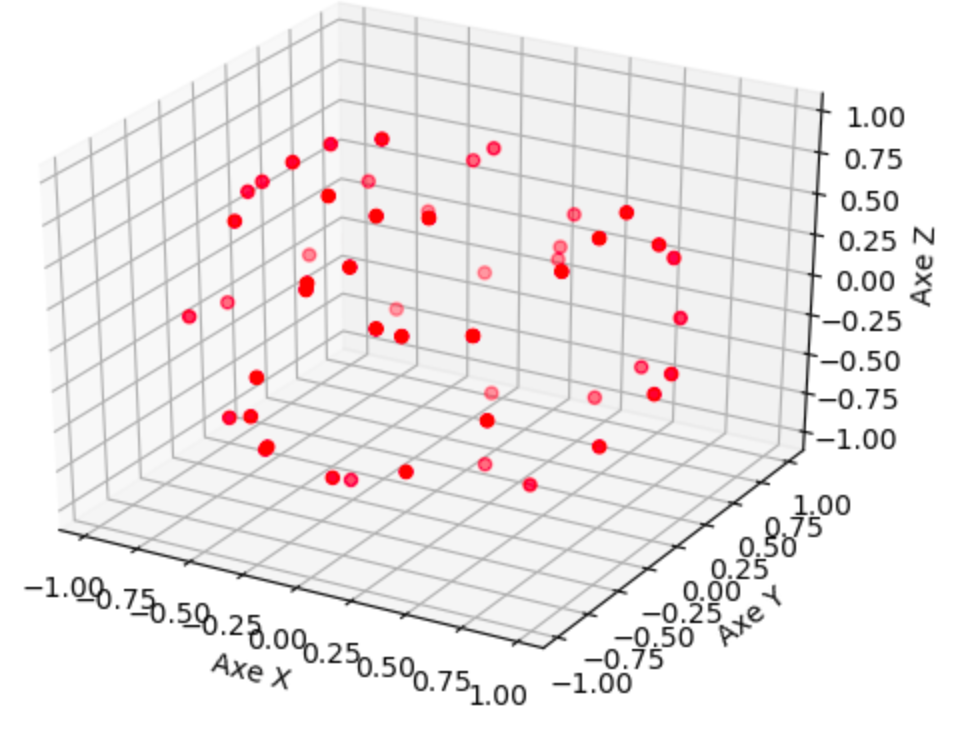
\includegraphics[width=0.8\columnwidth]{sampling_0.png}
  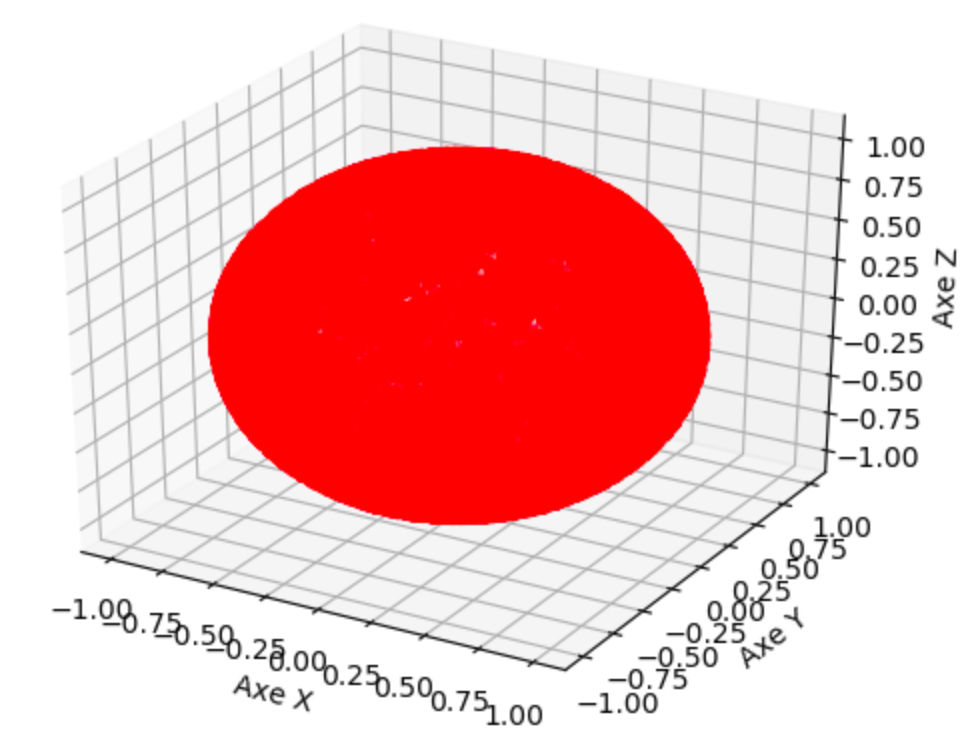
\includegraphics[width=0.8\columnwidth]{sampling_1.png}
  \end{multicols}
  \label{fig:samplings}
  \caption{Plot of the sampling of $\bm{v}_p$ for nMC = 50 and 10000 points.}
\end{figure}
\end{frame}



%\section{Regression testing

\begin{frame}{1D results}
\begin{figure}[h]
  \centering
  \begin{tikzpicture}
		\begin{axis}[%
			very thick,
			grid = both,
			major grid style = {lightgray},
			minor grid style = {lightgray!25},
			width = 0.9\textwidth,
			height = 0.7\textheight,
			xlabel = {x},
			ylabel = {Solution $u(x, t, v)$},
			legend style={at={(1,1)},anchor=north east},
            xmin = -1.0,
            xmax = 1.0,
            ymin = 0
			]
   
			\addplot[color=IBMblue, mark=none] table [col sep=space, x index=0, y index=3] {plot/solution_t_1.000000_nb_10.txt};
            \addplot[color=IBMorange, mark=none] table [col sep=space, x index=0, y index=3] {plot/solution_t_1.000000_nb_100.txt};
            \addplot[color=IBMpink, mark=none] table [col sep=space, x index=0, y index=3] {plot/solution_t_1.000000_nb_100000.txt};

        \legend{$\texttt{nbMC} = 10$,%
        $\texttt{nbMC} = 100$,
        $\texttt{nbMC} = 100000$,};
		\end{axis}
	\end{tikzpicture}
  \label{fig:visualisation1D}
  \caption{Solution refinement with \texttt{nbMC} in 1D.}
\end{figure}
\end{frame}

\begin{frame}{1D results}
\begin{figure}[h]
  \centering
  \begin{tikzpicture}
		\begin{axis}[%
			very thick,
			grid = both,
			major grid style = {lightgray},
			minor grid style = {lightgray!25},
			width = 0.9\textwidth,
			height = 0.7\textheight,
			xlabel = {t},
			ylabel = {Solution $u(0, t, v)$},
			legend style={at={(1,1)},anchor=north east},
            %xmin = -1.0,
            %xmax = 1.0,
            ymin = 0
			]

            \addplot[color=IBMorange, mark=none, domain=0:1] {5.0*exp(-x)}; 
			\addplot[color=IBMblue, mark=+, only marks, mark size=4pt] table [col sep=space, x index=0, y index=4] {plot/solution_depends_t.txt};

        \legend{$u_0 \e^{-|\bm{v}| \sigma_t t}$,$\texttt{nbMC} = 1000000$};
		\end{axis}
	\end{tikzpicture}
  \label{fig:visualisation_temps}
  \caption{Solution in 1D with $\sigma_s = 0$.}
\end{figure}
\end{frame}

\begin{frame}{1D results}
\begin{figure}[h]
  \centering
  \begin{multicols}{2}
  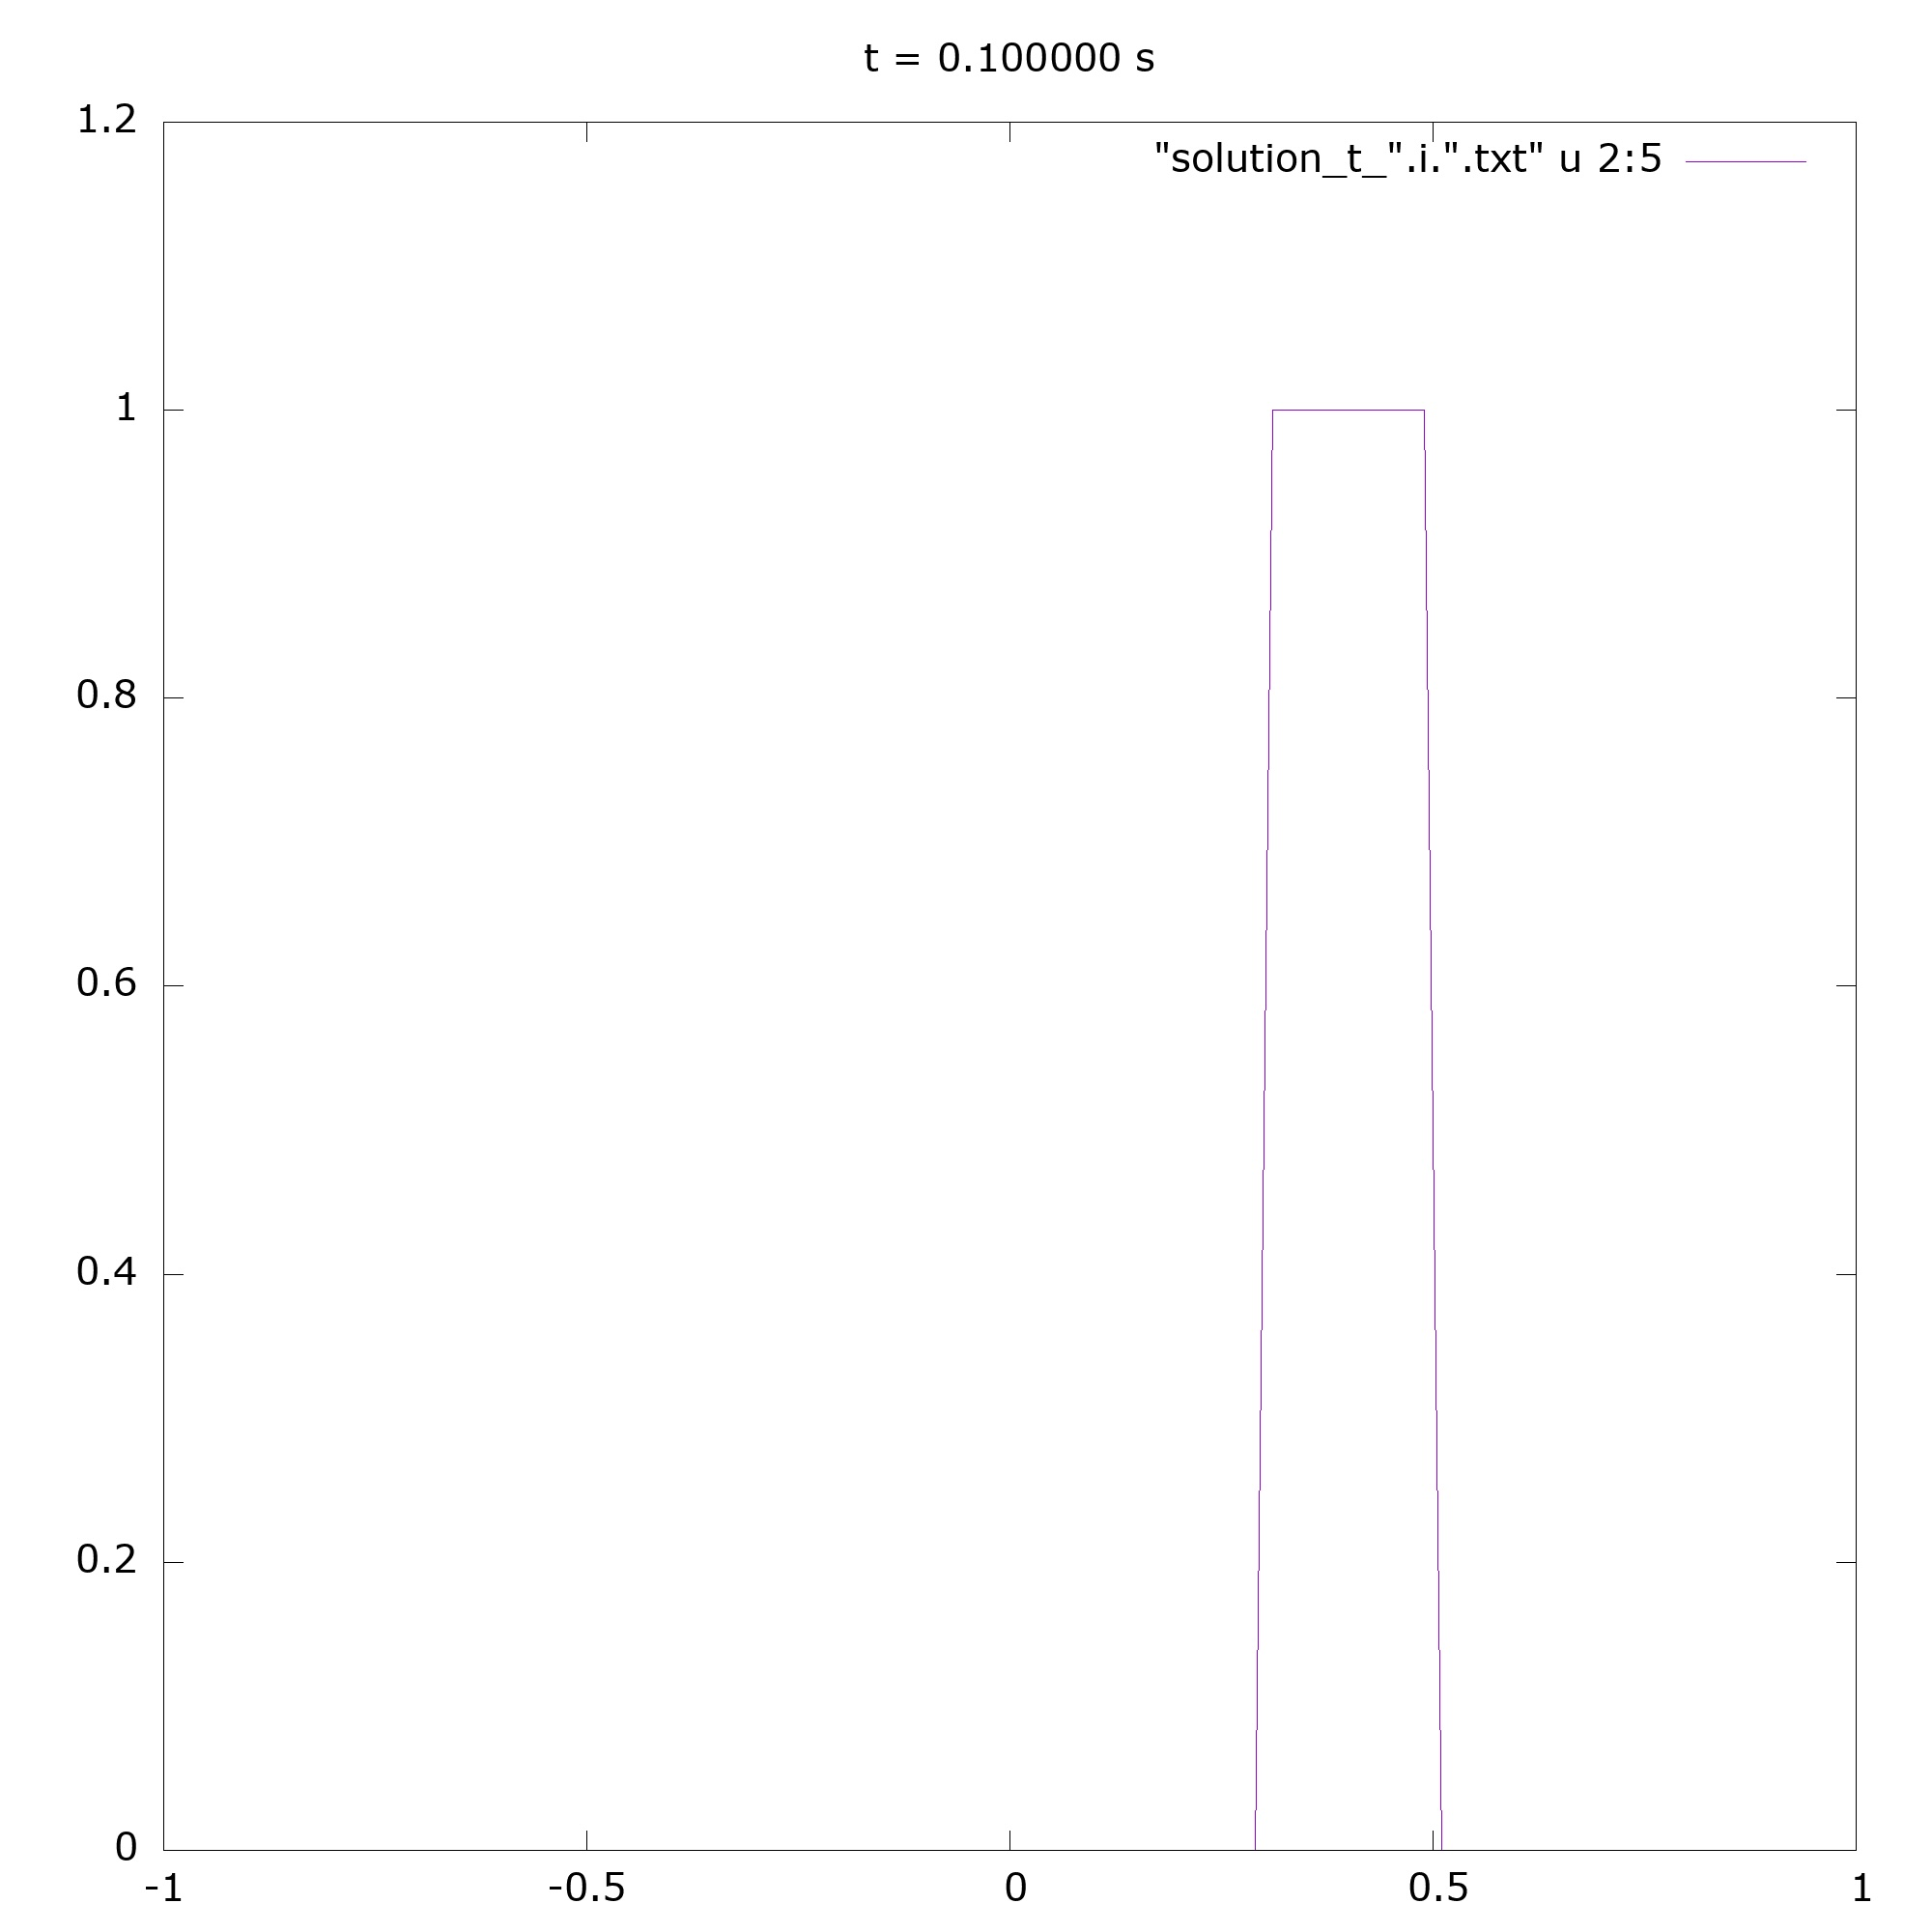
\includegraphics[width=0.8\columnwidth]{plot/advection.jpg}
  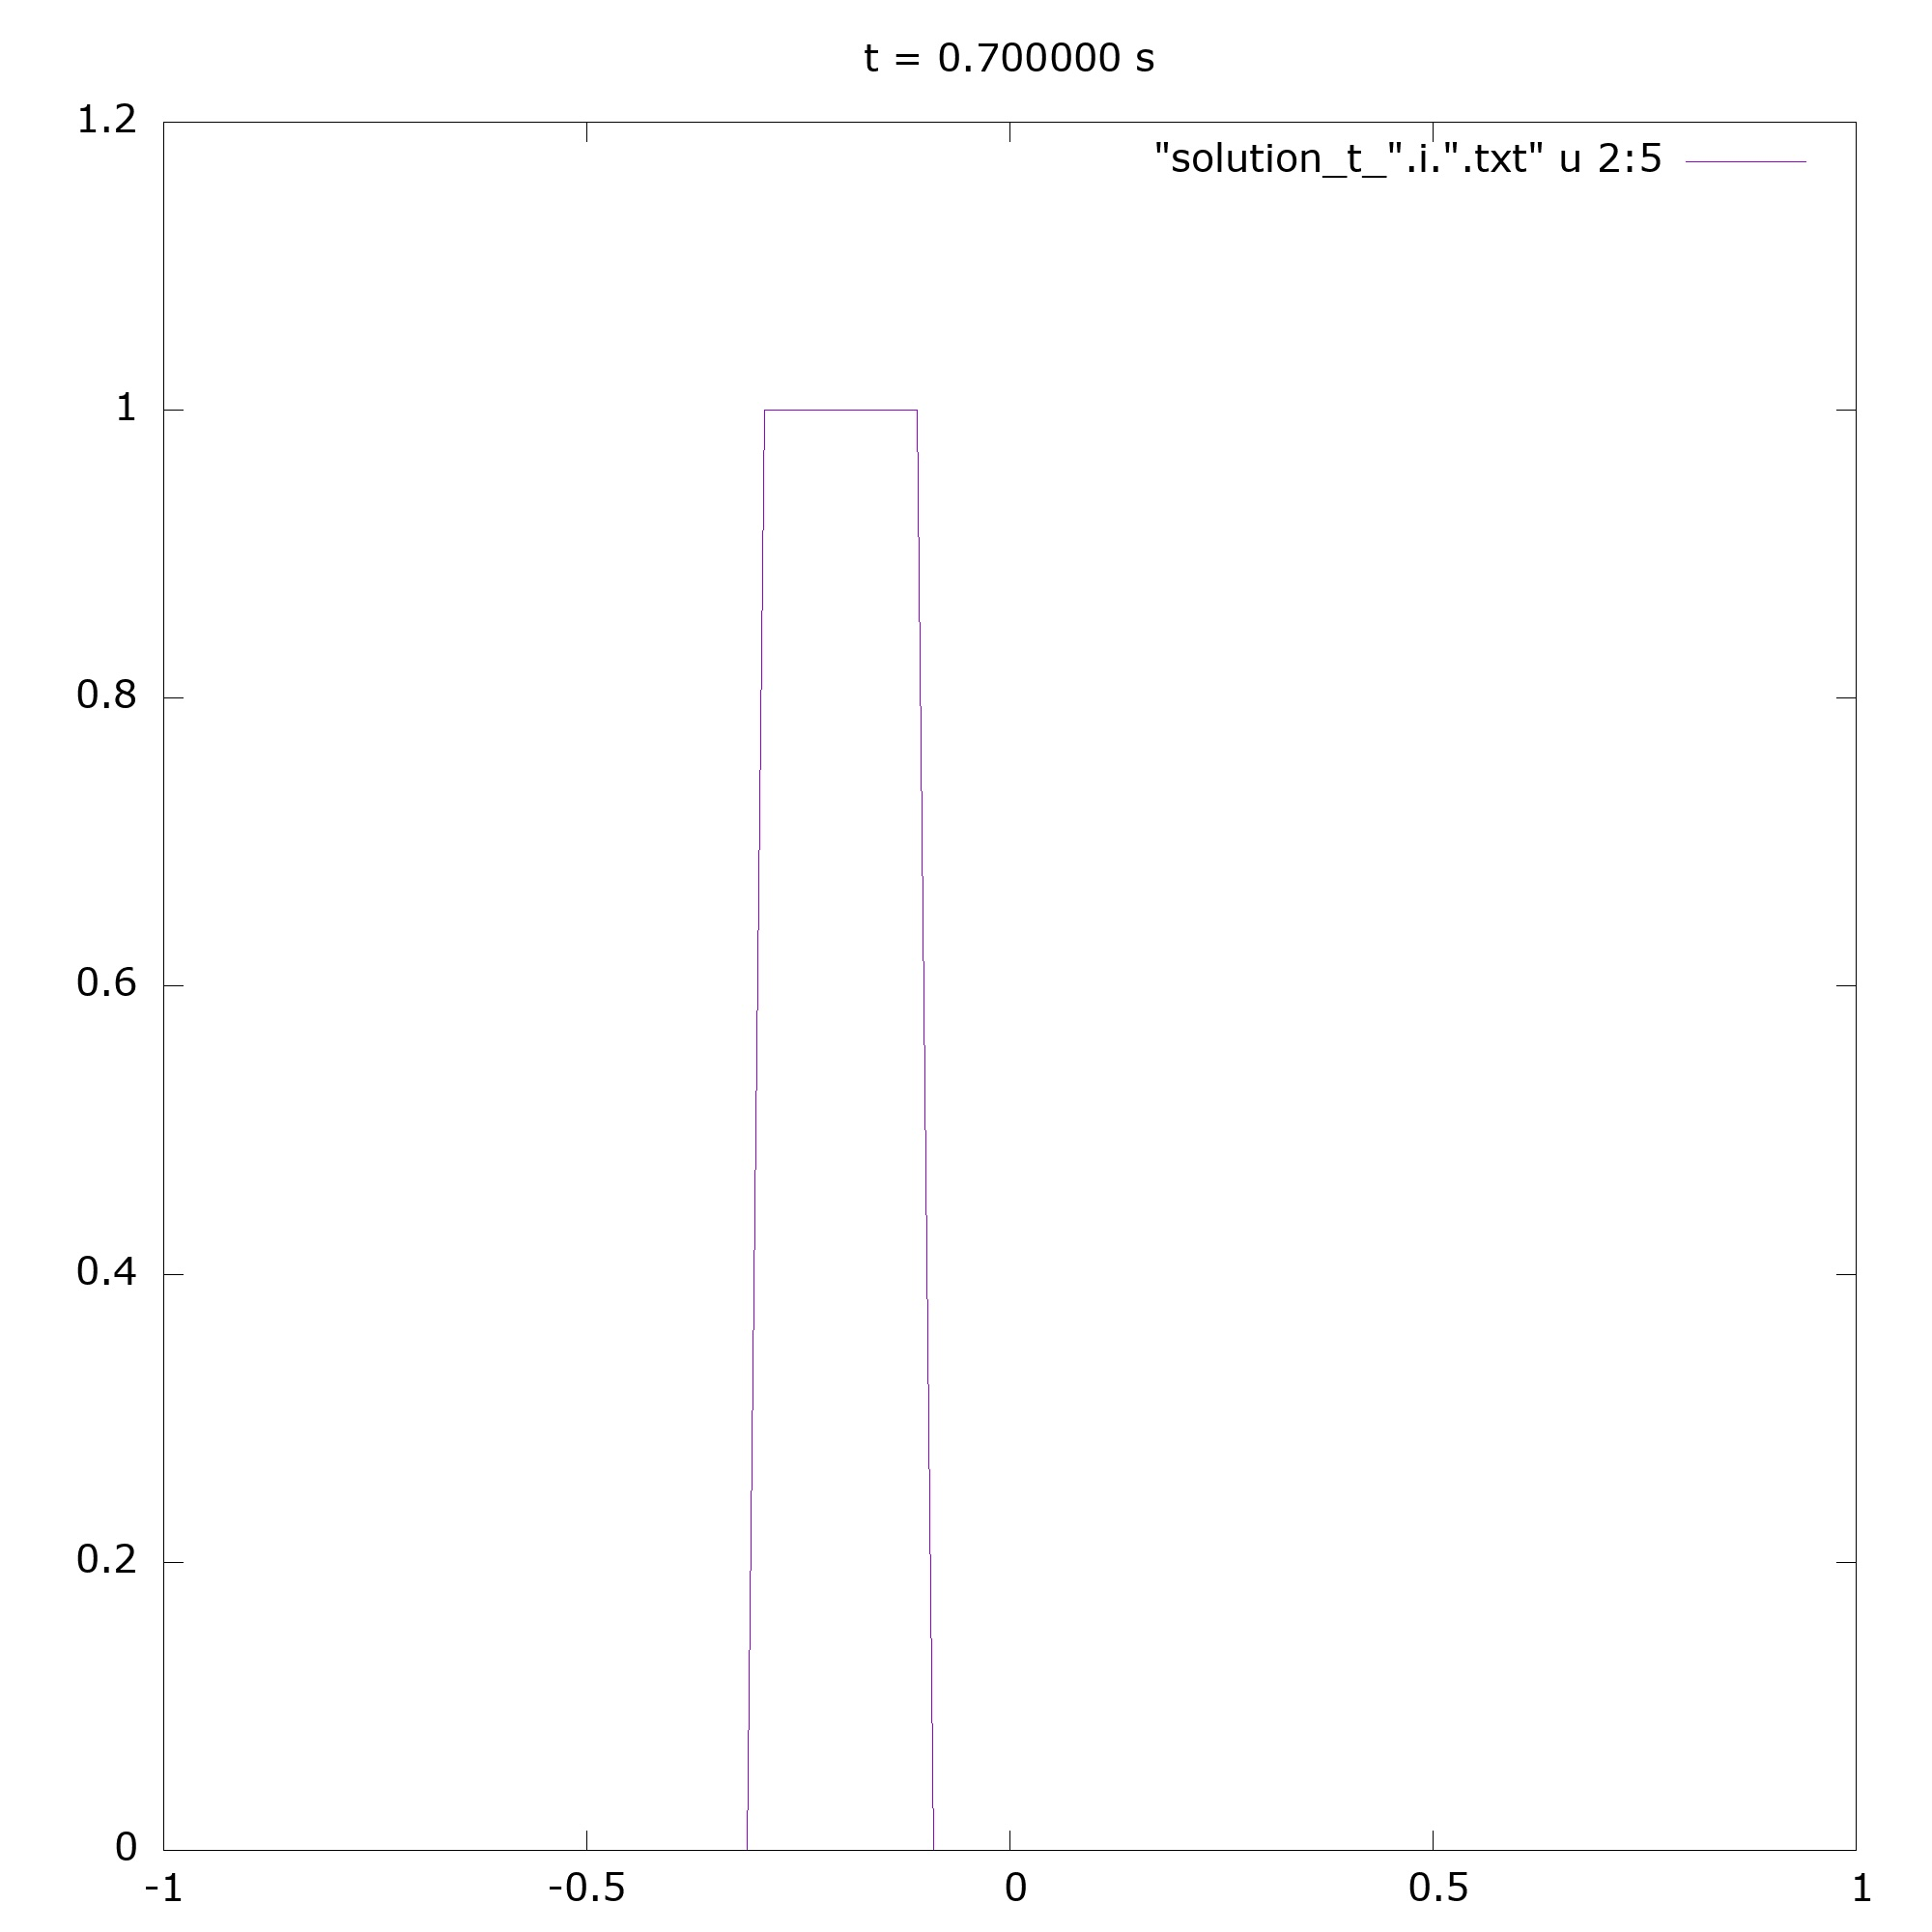
\includegraphics[width=0.8\columnwidth]{plot/advection1.jpg}
  \end{multicols}
  \label{fig:visualisation1D_temps}
  \caption{Solution in 1D with $\sigma_s = \sigma_t = 0$.}
\end{figure}
\end{frame}

\begin{frame}{2D result}
\begin{figure}[h]
  \centering
  \begin{tikzpicture}
		\begin{axis}[%
			%very thick,
			grid = both,
			major grid style = {lightgray},
			minor grid style = {lightgray!25},
			%width = 0.7\textwidth,
			height = 0.8\textheight,
			xlabel = {x},
			ylabel = {y},
            title = {Solution $u(\bm{x}, 1, v)$},
			legend style={at={(0.5,1)},anchor=north},
            xmin = -1.0,
            xmax = 1.0,
            ymin = -1.0,
            ymax = 1.0,
            view={0}{90},
            mesh/ordering=x varies,
            mesh/rows=20,
            colorbar,
            colormap/viridis,
            %shader=interp,
            %patch type=bilinear,
			]
   
			\addplot3 [color=IBMblue, surf] table [col sep=space, x index=0, y index=1, z index=3] {plot/solution_t_1.000000_2d.txt};

        \legend{$\texttt{nbMC} = 10$,};
		\end{axis}
	\end{tikzpicture}
  \label{fig:visualisation2D}
  \caption{\vspace{-1em}Solution in 2D with $20 \times 20$ points.}
\end{figure}
\end{frame}

\begin{frame}{References}
    \printbibliography
\end{frame}


\end{document}
